\documentclass[tikz,border=2pt]{standalone}
\usetikzlibrary{arrows.meta,positioning,calc,shapes.geometric}
\usepackage{fontspec}
\setmainfont{TeX Gyre Termes}
\setsansfont{Roboto}
\begin{document}
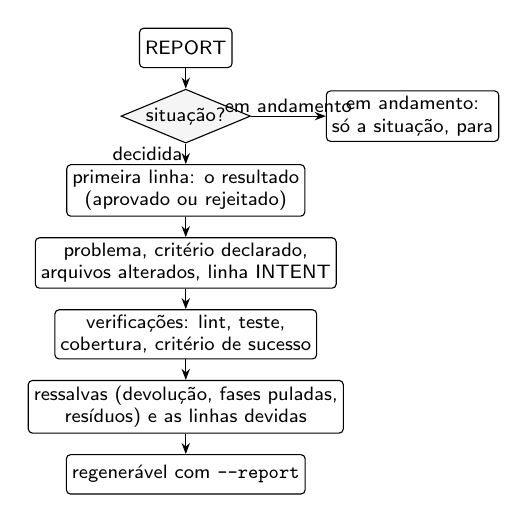
\begin{tikzpicture}[
  font=\sffamily\scriptsize, >={Stealth[length=4pt]},
  proc/.style={draw, thin, rounded corners=1.5pt, align=center, fill=white, minimum height=0.5cm, inner sep=2pt},
  dec/.style={draw, thin, diamond, aspect=2.4, align=center, fill=black!4, inner sep=0.5pt, font=\sffamily\scriptsize},
  nota/.style={font=\sffamily\scriptsize, align=center, text=black!80},
  lbl/.style={font=\sffamily\scriptsize, inner sep=1pt}
]
\node[proc] (a) {REPORT};
\node[dec, below=0.26cm of a] (st) {situação?};
\node[proc, right=0.95cm of st] (wip) {em andamento:\\ só a situação, para};
\node[proc, below=0.26cm of st] (first) {primeira linha: o resultado\\ (aprovado ou rejeitado)};
\node[proc, below=0.26cm of first] (body) {problema, critério declarado,\\
  arquivos alterados, linha INTENT};
\node[proc, below=0.26cm of body] (chk) {verificações: lint, teste,\\
  cobertura, critério de sucesso};
\node[proc, below=0.26cm of chk] (cav) {ressalvas (devolução, fases puladas,\\
  resíduos) e as linhas devidas};
\node[proc, below=0.26cm of cav] (n) {regenerável com \texttt{-{}-report}};
\draw[->] (a) -- (st);
\draw[->] (st) -- node[lbl,above]{em andamento} (wip);
\draw[->] (st) -- node[lbl,left]{decidida} (first);
\draw[->] (first) -- (body);
\draw[->] (body) -- (chk);
\draw[->] (chk) -- (cav);
\draw[->] (cav) -- (n);
\end{tikzpicture}
\end{document}
